\textbf{Higgs Decays to Invisible Particles, [PI: White]} \
A key question for the Higgs boson is whether it couples to the dark matter. 
If dark matter is indeed composed of particles, then presumably the 
125 GeV Higgs, or some other Higgs boson, is at least partially responsible 
for their mass generation (assuming that the new particles have a weak interaction).
We will continue to explore this possible connection by 
searching for evidence of Higgs decays to invisible particle(s).
Limits on the decay of the Higgs to invisible particles from the LHC experiments can be used in turn to set limits
on the process of dark matter particle-nucleon scattering, which are highly competitive with those from direct searches. 
The spin-independent cross-section for dark matter scattering on nucleons via Higgs exchange is directly related to the
invisible width of the Higgs.


The most promising channel for this analysis is Higgs production through Vector-Boson Fusion (VBF) 
as shown in Figure~\ref{fig:Higgs_VBF_diagram} (left). The signature for this process, with an invisible Higgs decay, 
is two forward jets, widely separated in pseudorapidity, and large missing transverse energy.
There is also a smaller signal contribution from gluon-fusion plus two jets.
The two main backgrounds are  $Z (\rightarrow \nu\nu)$ +jets and $W (\rightarrow \ell\nu) $ +jets (including $ \tau $ decays), 
where the charged-lepton in the final state is not identified in the detector. There are also
small backgrounds from the strong production of jets (multijet), t \tbar, and diboson production.
For the Run 1 analysis White served as contact editor together with Ketevi Assamagan(BNL), and Bill Quayle(LBNL). 
20.3 fb-1 of data at 8 TeV were analyzed and a limit of 28\% was set on the branching ratio of the H(125) to
 invisible particles at 95\% confidence level (with an expected limit of 31\%) ~\cite{HinvRun1}. This was the best limit set 
by all ATLAS and CMS analyses for Run 1. The use of a $W(\rightarrow \ell\nu) $ control region, as well as the
$Z (\rightarrow \ell\ell) $ control region, to estimate the $Z (\rightarrow \nu\nu) $ +jets background was a 
significant factor in setting our low Run 1 limit. Figure~\ref{fig:Higgs_VBF_diagram} (right) also shows the limit, as a function of mass, 
that our analysis sets on the Higgs-nucleon cross-section, and the comparison with direct search limits. 
White presented the ATLAS and CMS results on invisible decays of the Higgs at the LHCP2015 Conference in St. Petersburg, Russia. ~\cite{LHCP2015}

\begin{figure}[htb]
\centering

      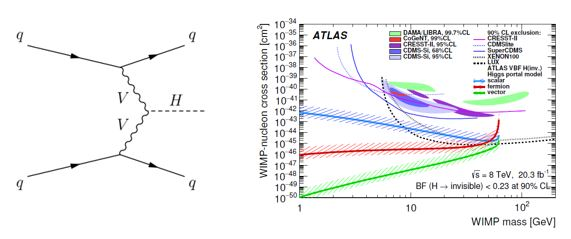
\includegraphics[scale=0.8]{Figures/Higgs_VBF_diagram.jpg}
      \label{fig:Higgs_VBF_diagram}

\caption{(left) Vector-Boson Fusion. (right) WIMP nucleon cross section as a function of the WIMP mass.}
\end{figure}


The increased Higgs production cross-section at 13 \TeV, and the higher integrated luminosity from Run 2 will allow us to probe this process
with significantly increased sensitivity over our Run 1 results. White (working with Alex Madsen (DESY)) is analysis contact for the
Run 2 Higgs to Invisible analysis. Weekly meetings are held to coordinate the contributions to the analysis: data/Monte Carlo samples and 
comparisons, trigger(s), control regions specification, theory uncertainties, and limit setting. We have also been holding workshops 
at critical times to advance the analysis. 
Given the rate at which ATLAS is acquiring integrated luminosity, we expect in 2016 to reach the point at which we begin to be limited by 
systematic errors rather than statistically limited. In this respect investigations are ongoing into potential methods
for cancellation of systematics in efficiency ratios versus the usual application of transfer factors from control to signal regions.
Specific contributions from UTA to the Run 2 analysis include calculating the electroweak corrections to the the VBF Higgs signal, and
providing the parton distribution function (pdf) uncertainties on the signal. For the electroweak corrections, we have set up HAWK ~\cite{HAWK} 
on the UTA Tier 3 in multi-threaded 
mode as more than $10^{9}$ events are needed to achieve sufficiently precise corrections. HAWK provides the calculation of differential 
EW correction factors, which can be used as differential EW reweighting factors to improve QCD-based predictions. The results of the HAWK
calculations are shown in Figure~\ref{fig:HAWK_EW} - the reweighting factors have essentially a linear dependence on the Higgs Pt, and a linear fit
yields the required electroweak correction. 

\begin{figure}[htb]
\centering

      \includegraphics[scale=0.5]{Figures/HAWK_EW.jpg}
      \label{fig:HAWK_EW}

\caption{Electroweak corrections to the Higgs pT distribution in the VBF selection.}
\end{figure}

For the calculation of the VBF signal pdf uncertainties, UTA has been running the generator Powheg v.2 ~\cite{Powheg} which allows the storage of
multiple weights for each event. Our original VBF signal dataset was created using the CT10 pdf set. There are now recommended pdf 
sets for LHC Run 2 which combine CT14, MMHT2014, and NNPDF3.0 ~\cite{Run2PDF}. Currently, after exchanges with Higgs and Exotics group colleagues 
we have chosen to use the PDF4LHC15-nlo-30-pdfas set. This is a Hessian set that allows straightforward calculation of the 
uncertainties, which is the variation in the number of weighted events passing the VBF selection. This work is being carried out 
by UTA Honors undergraduate student Darshan Chalise under White's direction. UTA will continue to provide both the electroweak and 
pdf uncertainties for future versions of our analysis.
  
The current analysis plan is to write a paper based on the 2015-16 data set, estimated to comprise about 30 fb$^{-1}$. The goal is to have 
this result ready for Moriond 2017. White will take on a new graduate student in the Fall 2016 semester. This student will work on the
2017-18 extension of the VBF Higgs to Invisible analysis. Going forward we will focus on improvements and changes to the analysis that
will be necessitated by the rising instantaneous luminosity - pileup mitigation, particularly for forward jets, and reduction of the
systematics for the jet energy scale and resolution. Work in these areas will form part of White's new student's ATLAS qualification 
tasks. Of significant physics interest, with reducing limits on the Higgs to invisible branching ratio, will be our ability to exclude 
models that predict an enhanced value of this ratio. There is a natural evolution of White's physics interest in this topic also with the ILC project (see the ILC
 section below), which will allow much stronger constraints to be set on Higgs to invisible decays.

\textbf{VBF HIggs to Invisible Analysis Timetable of Activities}

\textbf{2017}
\begin{itemize}[noitemsep,nolistsep]
\item{New UTA graduate student starts work on ATLAS}
\item{Publish Run 2 paper based on 2015-16 dataset}
\item{Work on "interpretation" paper for Run 2 results, DM-nucleon limits and more}
\item{Study strategies for reduction of jet systematics}
\item{Update Higgs to Invisible limit as more data becomes available}
\end{itemize}

\textbf{2018}
\begin{itemize}[noitemsep,nolistsep]
\item{Graduate student pursues ATLAS qualification with work on strategies for reduction of jet systematics}
\item{Contribute data/MC comparisons and cutflow checks}
\item{Provide updated electroweak signal corrections, and pdf uncertainties}
\item{Graduate student begins year at CERN}
\item{Work on branching ratio limit from full Run 2 dataset}
\end{itemize}

\textbf{2019}
\begin{itemize}[noitemsep,nolistsep]
\item{Publish full Run 2 result}
\item{Work on analysis strategies beyond Run 2}
\end{itemize}
